\documentclass{standalone} %tipo de documento "imagens solo".

\usepackage{tikz} %para imagens e gráficos vetoriais

\usepackage{circuitikz} %para desenhar circuitos elétricos

\usepackage{tkz-euclide} %define pontos no plano cartesiano

\begin{document}

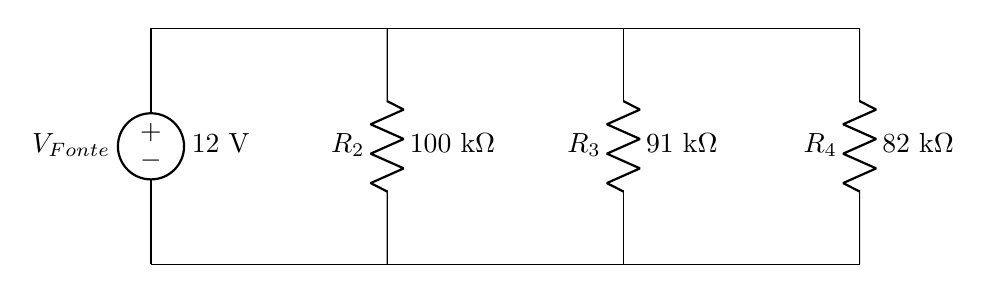
\begin{tikzpicture}[american] %define a tipologia dos componentes do circuito

%O comando \tkzDefPoints define os pontos no plano cartesiano para facilitar o posicionamento dos componentes do circuito. Os pontos são definidos pelas coordenadas (x/y/NomedoPonto)
\tkzDefPoints{
-8/5/A,
-8/2/B,
-5/5/C,
-5/2/D,
-2/5/E,
-2/2/F,
1/5/G,
1/2/H}

%Do ponto (-8,5) ao ponto (-8,2) cria um segmento com um resistor (vsource) no centro. Teste o comando "a" e "l" para incluir o rótulo do resistor, dentro ou fora do elemento. 
%---------------------------------------------------
\draw (A) to [vsource, a=$V_{Fonte}$, l=$12$ V] (B);
%---------------------------------------------------

%Do ponto (-5,5) ao ponto (-5,2) cria um segmento com um resistor (R) no centro. Teste o comando "a" e "l" para incluir o rótulo do resistor, dentro ou fora do elemento. 
%---------------------------------------------------
\draw (C) to [R, a=$R_{2}$, l=$100$ k$\Omega$] (D);
%---------------------------------------------------

%Do ponto (-2,5) ao ponto (-2,2) cria um segmento com um resistor (R) no centro. Teste o comando "a" e "l" para incluir o rótulo do resistor, dentro ou fora do elemento. 
%---------------------------------------------------
\draw (E) to [R, a=$R_{3}$, l=$91$ k$\Omega$] (F);
%---------------------------------------------------

%Do ponto (1,5) ao ponto (1,2) cria um segmento com um resistor (R) no centro. Teste o comando "a" e "l" para incluir o rótulo do resistor, dentro ou fora do elemento. 
%---------------------------------------------------
\draw (G) to [R, a=$R_{4}$, l=$82$ k$\Omega$] (H);
%---------------------------------------------------

%---------------------------------------------------
%Conectando os segmentos não preenchidos
%---------------------------------------------------

%Do ponto (-8,5) ao ponto (-5,5) cria um segmento "short".
%---------------------------------------------------
\draw (A)--(C);

%Do ponto (-5,5) ao ponto (-2,5) cria um segmento "short".
%---------------------------------------------------
\draw (C)--(E);

%Do ponto (-2,5) ao ponto (1,5) cria um segmento "short".
%---------------------------------------------------
\draw (E)--(G);

%Do ponto (1,2) ao ponto (-2,2) cria um segmento "short".
%---------------------------------------------------
\draw (H)--(F);

%Do ponto (-2,2) ao ponto (-5,2) cria um segmento "short".
%---------------------------------------------------
\draw (F)--(D);

%Do ponto (-5,2) ao ponto (-8,2) cria um segmento "short".
%---------------------------------------------------
\draw (D)--(B);

\end{tikzpicture}

\end{document}
